\documentclass[12pt]{article}
\usepackage{graphicx,float}
\usepackage{listings}
\usepackage{xcolor}
\graphicspath{{./fig/}}

\definecolor{codegreen}{rgb}{0,0.6,0}
\definecolor{codegray}{rgb}{0.5,0.5,0.5}
\definecolor{codepurple}{rgb}{0.58,0,0.82}
\definecolor{backcolour}{rgb}{0.95,0.95,0.92}


\lstdefinelanguage{SPICE}{
  keywords={tran,ac,dc,subckt,meas,plot,print,control,run,end,endc, hardcopy},
  morecomment=[l]{*},
  morecomment=[l]{\$},
  morecomment=[s]{/*}{*/},
  morestring=[b]',
  morestring=[b]",
  ndkeywords={r,r1,r2,r3,r4,r5,l,l1,l2,l3,l4,l5,c,c1,c2,c3,c4,c5,v,vin,m,m1,m2,m3,m4,m5,d,d1,d2,d3,d4,d5,vdb, pulse,sin,i,pwl,exp},
  keywordstyle=\color{blue}\bfseries,
  ndkeywordstyle=\color{codegreen}\bfseries,
  identifierstyle=\color{black},
  commentstyle=\color{purple}\ttfamily,
  stringstyle=\color{red}\ttfamily,
  sensitive=true
}

\lstdefinestyle{mystyle}{
	backgroundcolor=\color{backcolour},   
    commentstyle=\color{codegreen},
    keywordstyle=\color{magenta},
    numberstyle=\tiny\color{codegray},
    stringstyle=\color{codepurple},
    basicstyle=\ttfamily\footnotesize,
    breakatwhitespace=false,         
    breaklines=true,                 
    captionpos=b,                    
    keepspaces=true,                 
    numbers=left,                    
    numbersep=5pt,                  
    showspaces=false,                
    showstringspaces=false,
    showtabs=false,                  
    tabsize=4
}

\lstset{style=mystyle}


% Title[Enter title of the experiment here]
\title{EE230: Lab-3\\
Circuits using OP-AMPS}

% Author[Enter details of author here]
\author{Prateek Garg, 20D070060}

% begin the document.
\begin{document}
\noindent
% make a title page.[this creates title page]
\maketitle

\section{Overview of the experiment} %[This segment creates Section as seen in document]

\subsection{Aim of the experiment}%[This segment creates sebsections under the same section]
The im of the experiment is to study and simulate various opamp circuits in ngspice namely: 
\begin{enumerate}
    \item Schmidt Trigger
    \item Astable Multivibrator
    \item Monostable Multivibrator
\end{enumerate}
\subsection{Methods}
We start by analysing the circuits and then simulating in ngspice to check against theoretical expectations.  
\section{Design}
%Add circuit Diagrams here
%With accompaying Explanantions 
\subsection{Schmidt Trigger}
\begin{figure}[H]
  \begin{center}
    \makebox{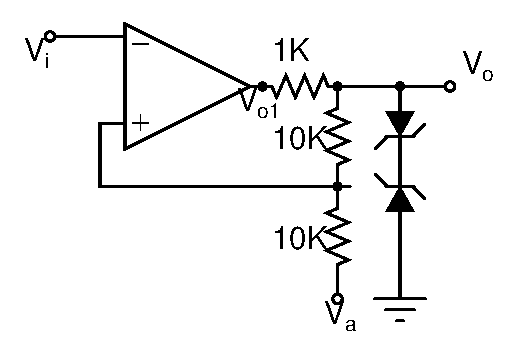
\includegraphics{Schimdttrigger.eps}}
\end{center}
\end{figure}

\subsection{Astable Multivibrator}
\begin{figure}[H]
  \begin{center}
    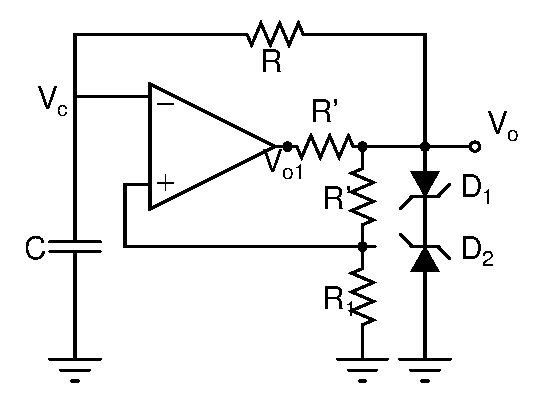
\includegraphics{Astable_Multivibrator.eps}
\end{center}
\end{figure}

\subsection{Monostable Multivibrator}
\begin{figure}[H]
  \begin{center}
    \includegraphics{Monostable_Multivibrator.eps}
\end{center}
\end{figure}

\section{Simulation results}

\subsection{Schimdt Trigger}
\subsubsection{Code snippet}
\lstinputlisting[language=SPICE]{../Schmitt_trigger.cir}
\subsubsection{Simulation results}
%\makebox[\textwidth]{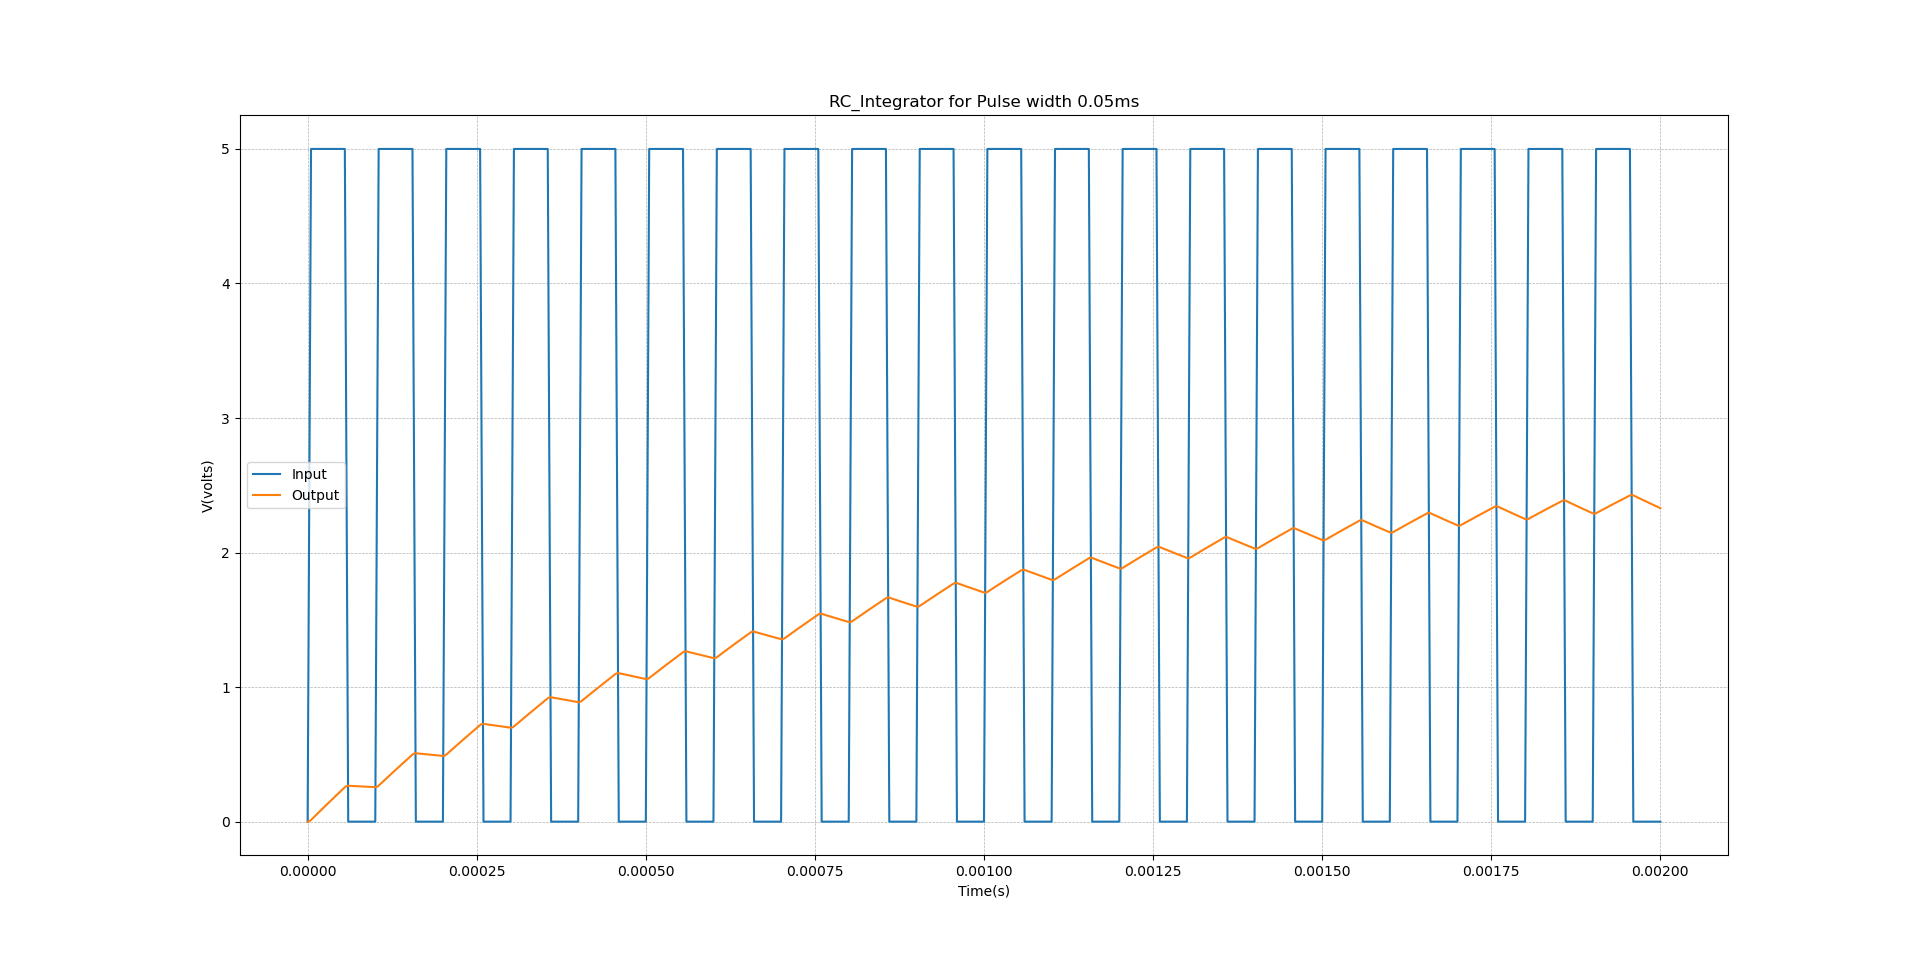
\includegraphics[width=\paperwidth]{RC_Integrator_6.png}}

\subsection{Astable Multivibrator}
\subsubsection{Code snippet}
\lstinputlisting[language=SPICE]{../Astable_Multivibrator-1.cir}
\subsection{Monostable Multivibrator}
\subsubsection{Code snippet}
\lstinputlisting[language=SPICE]{../Monostable_Multivibrator.cir}


\subsubsection{Simulation results}
\textbf{\large Schimdt Trigger}
\begin{figure}[H]
  \begin{center}
    \makebox[0.8\textwidth]{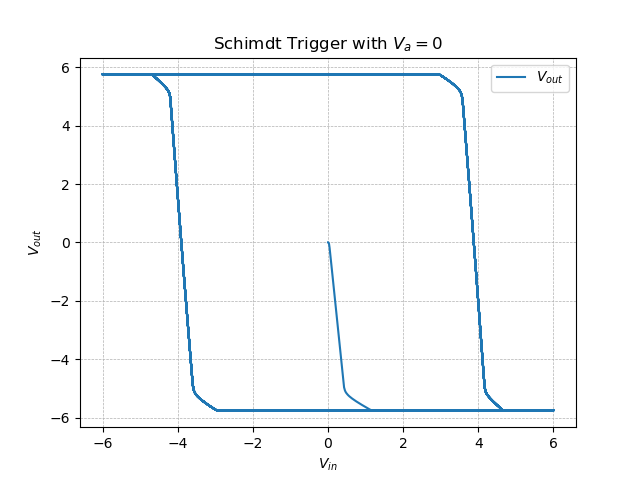
\includegraphics[width=0.8\paperwidth]{Schimdt-Trigger-with-Va=0.png}}
\end{center}
\end{figure}

\begin{figure}[H]
    \begin{center}
      \makebox[0.8\textwidth]{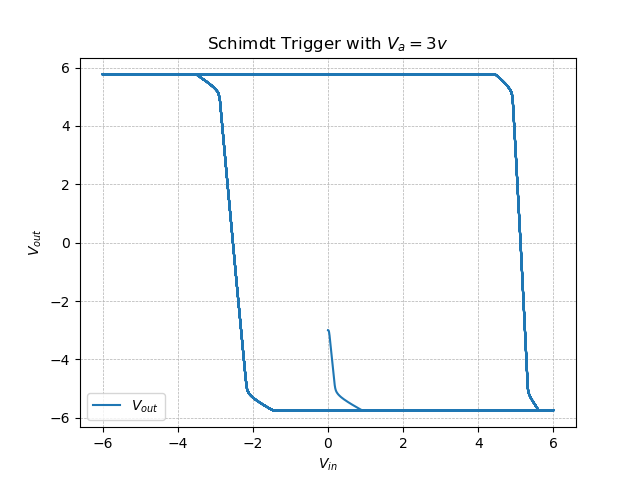
\includegraphics[width=0.8\paperwidth]{Schimdt-Trigger-with-Va=3v.png}}
\end{center}
\end{figure}

\begin{figure}[H]
    \begin{center}
      \makebox[0.8\textwidth]{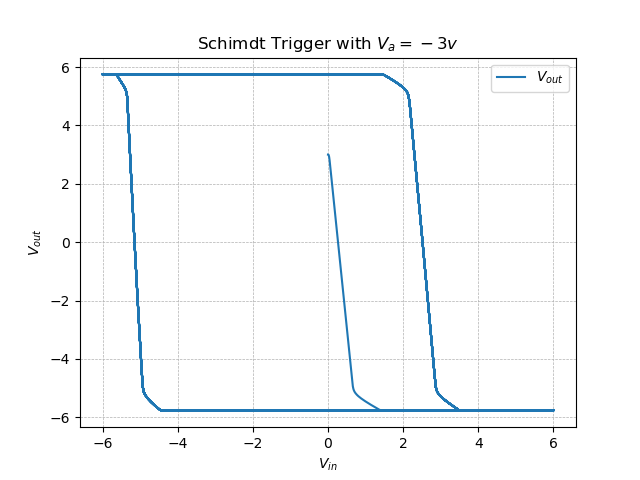
\includegraphics[width=0.8\paperwidth]{Schimdt-Trigger-with-Va=-3v.png}}
  \end{center}
\end{figure}    

\textbf{\large Astable Multivibrator}
\begin{figure}[H]
  \begin{center}
    \makebox[0.8\textwidth]{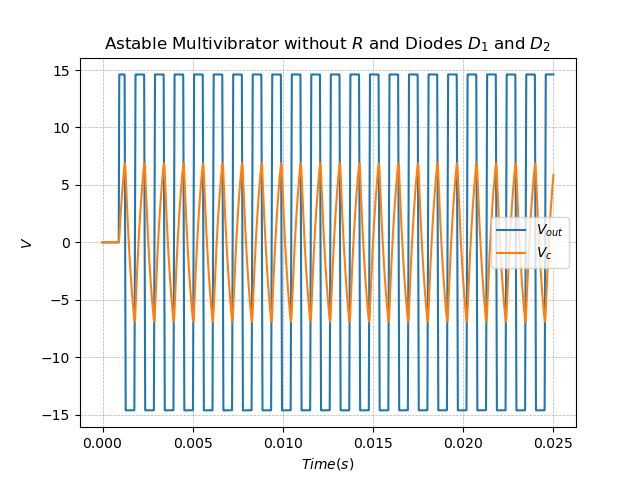
\includegraphics[width=0.8\paperwidth]{Astable-Multivibrator-without-R-and-Diodes-D1-and-D2.png}}
\end{center}
\end{figure}

\begin{figure}[H]
    \begin{center}
      \makebox[0.8\textwidth]{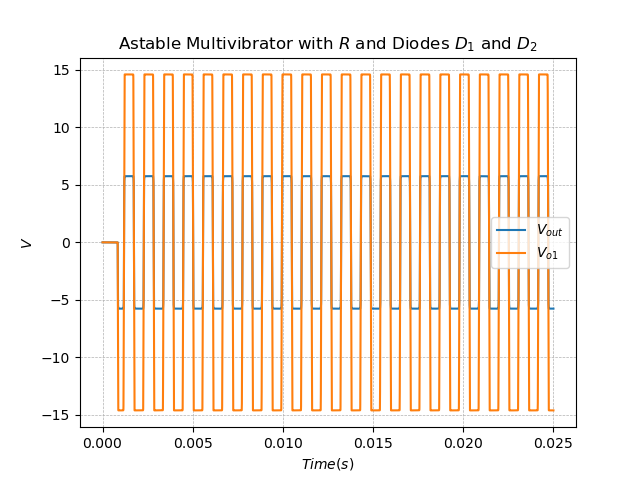
\includegraphics[width=0.8\paperwidth]{Astable-Multivibrator-with-R-and-Diodes-D1-and-D2.png}}
  \end{center}
  \end{figure}

  \textbf{\large Monostable Multivibrator}
  \begin{figure}[H]
    \begin{center}
      \makebox[0.8\textwidth]{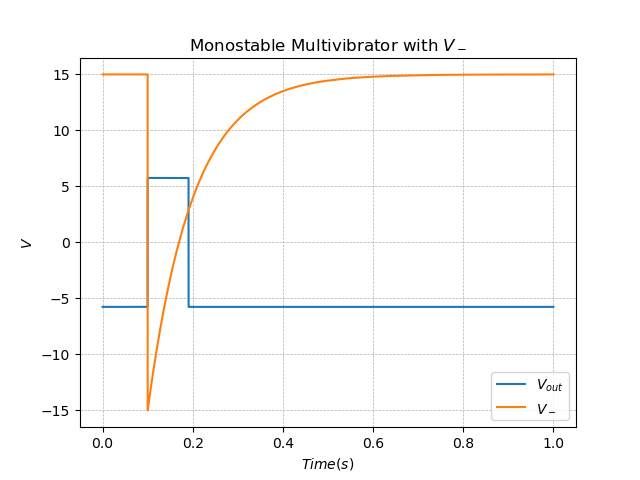
\includegraphics[width=0.8\paperwidth]{Monostable-Multivibrator-with-V-.png}}
  \end{center}
  \end{figure}

\section{Experiment completion status}
All the sections were completed
\end{document}
